% Author: David Paulino
% Date: 2023-03-03
% Description: LaTeX Template


\documentclass[12pt]{article}

% Document en français
\usepackage[french]{babel}

\usepackage[utf8]{inputenc}
\usepackage[T1]{fontenc}
\usepackage{graphicx}
\usepackage{amsmath}
\usepackage{amssymb}
\usepackage{amsthm}
\usepackage{amsfonts}
\usepackage{amscd}
\usepackage{amstext}

\usepackage{hyperref}
\usepackage{xcolor}
\usepackage{fancyhdr}
\usepackage{setspace}
\usepackage{float}
\usepackage{subfig}
\usepackage{caption}
\usepackage{listings}
\usepackage{tikz}
\usepackage{pgfplots}
\usepackage{pgfplotstable}
\usepackage{pgf}

% Add references in table of contents
\usepackage[nottoc]{tocbibind}

% Set author and place
\newcommand{\DP}{David Paulino}
\newcommand{\place}{Genève}
\newcommand{\fulltitle}{Analyse et optimisation de l'expected goal: application au machine learning}
\newcommand{\shorttitle}{Analyse et optimisation de l'expected goal}

% Title
\title{Title}
\author{\DP}
\date{\today}

% Header
\pagestyle{fancy}
\fancyhf{}
\renewcommand{\headrulewidth}{0pt}
\lhead{\DP}
\rhead{\shorttitle}

% Footers
\lfoot{Page \thepage}
\rfoot{\today}

% Document
\begin{document}

% Title page
\begin{titlepage}

    \begin{figure}[h]
        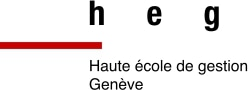
\includegraphics[width=0.3\textwidth]{img/logo_heg-ge.jpg}
    \end{figure}

    \vspace*{0.5cm}

    \begin{center}

        \begingroup \linespread{1,75} \selectfont
        {\Large \fulltitle}\\[0,75cm]
        \endgroup


        % Make a vertical space

        \vspace{1.5cm}

        \textsc{\large Travail de Bachelor HES réalisé en vue de \newline l’obtention du Bachelor par :}\\[0,50cm]

        \begingroup \linespread{1,5} \selectfont
        \textsc{\large \DP}\\[0,50cm]
        \endgroup


        \vspace{1cm}


        \textsc{\large Conseillers au travail de Bachelor : }

        \begingroup \linespread{1,5} \selectfont
        \textsc{\large Pr Alexandros KALOUSIS}\\[0.1cm]
        \textsc{\large Dr Nils SCHÄTTI}\\[1cm]
        \endgroup


        \begingroup \linespread{1,75} \selectfont
        \textsc{\large \place, le \today}\\[0,1cm]

        {\large Haute école de Gestion de Genève (HEG-GE)}\\[0,1cm]

        {\large Filière Informatique de gestion}\\[0,1cm]
        \endgroup



        \begin{figure}[h]
            \vspace{0.05cm}
            \hspace*{12cm}
\includegraphics[width=0.25\textwidth]{img/logo_hes-so.jpg}
        \end{figure}

    \end{center}



    \vfill
\end{titlepage}




\newpage

% Table of contents
\tableofcontents
\newpage

% Content
\section{Introduction}

% Citation avec Zotero et BibLaTeX
\subsection{Introduction à la problématique}
\noindent Lorsque les premiers sports sont apparus, l'information la plus importante était le score et le vainqueur de la confrontation.
Au fur et à mesure, plus d'informations sur les matchs sont venues s'ajoutées.
Le nombre de tirs dans un matchs par équipes, le nombre de passes, le nombre de tirs cadrés, la possession du ballon le pourcentage de passes réussies dans le football, le nombre de passes décisives et d'autres sont venus s'ajouter aux statistiques dans le football.
Le pourcentage de réussite aux lancers francs, le nombre de rebonds, le nombre de passes décisives, le pourcentage de réussite aux tirs, le nombre de fautes, le nombre de minutes jouées, le pourcentage de réussite à 3 points et d'autres sont venus s'ajouter aux statistiques dans le basketball.
Ces statistiques sont également devenus personnelles à chacun des joueurs.
On peut également compter pour le baseball le nombre de fois qu'un joueur était au bâton, son nombre de double, de triples, son nombre de buts et bien d'autres.
\newline\newline
C'est d'ailleurs dans le baseball que l'on peut retrouver la première utilisation de statistiques avancées pour établir des stratégies.
En effet, au début des années 1970, le joueur des Baltimore Orioles a développé une analyse statistiques pour choisir le meilleur alignement possible pour son équipe de départ.
Cependant, il n'a pas pu l'utiliser à ce moment-là puisque le président de sa franchise n'avait pas confiance. C'est qu'à partir de 1984 où il fut le coach des New York Mets qu'il a pu mettre en place son analyse statistiques avancées pour établir le meilleur choix pour son équipe de départ. \cite{incPCMag1984}
Deux saisons plus tard, il remporte la Série mondiale 1986 \footnote{En MLB, la Série mondiale est la série finale qui permet de déterminer qui est l'équipe championne de la ligue.}. Les Mets étaient situés à la dernière place de leur conférence avant l'arrivée de Davey Johnson et son management orienté sur les statistiques.
\newline
Après cette réussite, les autres franchises de la MLB\footnote{Ligue majeure de baseball} ont également commencé à adopter l'analyse de statistiques dans le sport et cela a également été populaire dans les autres sports avec par exemple Daryl Morey qui a été le premier coach analyste statistiques recruté chez les Rockets de Houston en NBA en 2007. \cite{DarylMorey13year2020}
Les franchises de la NBA\footnote{Ligue nationale de basketball} ont par la suite également adopté une approche managériale statistique.
On constate alors que cette culture de la statistique dans le sport provient des États-Unis.
\newline
Il est désormais important d'amener l'arrivée des expected goals. L'une des premières études sur un modèle d'expected goals vient d'Alan Ryder qui a publié une étude sur la qualité des tirs effectuées dans des matchs de hockey. \cite{ryderIsolatingShotQuality2004}
Ce dernier a pu analyser les différentes circonstances lors d'un tir et développer un modèle qui prédit la probabilité d'un tir selon les circonstances de ce tir.
Dans le football, l'une des premieres études sur l'expected goal vient de Richard Pollard, Jake Ensum et Samuel Taylor qui ont analysé les facteurs qui influent la chance de marquer un but. \cite{pollardEstimatingProbabilityShot2004} La problématique de ce travail est donc de pouvoir analyser et optimiser l'expected goal.
\newline\newline
Il semble maintenant important de savoir ce qu'est l'expected goal. L'expected goal
\footnote{Très souvent réduit par xG} est une métrique qui permet de déterminer la probabilité qu'un tir soit transformé en but selon les données de ce tir \cite{XGExplainedFBrefa}.
Un tir qui a un xG de 0.4 a une probabilité de 40\% d'être transformé en but. Un tir avec un xG à 1 est la plus grande valeur possible et aurait donc 100\% de chance d'être transformé en but.
\footnote{Il est important d'indiquer qu'il est très rare qu'un xG d'un tir soit égal à 1 mais il va généralement s'en rapprocher fortement selon ses paramètres.} \cite{pettyWhatExpectedGoals2018a}
\newline\newline
Pour observer ce qu'est réellement un xG, nous allons l'observer avec l'emplacement de deux tirs sur un terrain.
Le schéma \ref{fig:expected_goal_example} montre un terrain de football avec deux emplacements de tirs.
Par exemple, le tir en rouge aurait un xG de 0.1 et le tir en vert aurait un xG de 0.5\footnote{Ces métriques sont que des exemples et n'ont pas été produites par un modèle.}.
\newline \newline
\noindent Par ailleurs, les xG se sont tellement développés que des métriques dérivées ont été créées. On peut par exemple citer le xA qui est l'expected assist. C'est une métrique qui permet de déterminer la probabilité qu'une passe soit transformée en passe décisive selon les données de cette passe. \cite{XGExplainedFBrefa}
Également, les xGA qui est les expected goals against. Cette métrique permet de déterminer la probabilité qu'un tir soit transformé en but selon les données de ce tir mais pour l'équipe adverse. \cite{pettyWhatExpectedGoals2018a}

\noindent Il y en a également d'autres comme les expected points qui sont les points qui est le nombre de points qu'une équipe devrait avoir gagnés basé sur les données relatives aux xG. D'autres dérivées sont indiquées sur l'article de Pinnacle écrit par Luke Petty. \cite{pettyWhatExpectedGoals2018a}
\newline\newline
\noindent Maintenant que nous avons vu ce qu'est un xG et ces dérivées actuelles, il semble pertinent de décrire l'utilisation de cette métrique dans le football actuel.

\begin{figure}[htp]
    \centering
    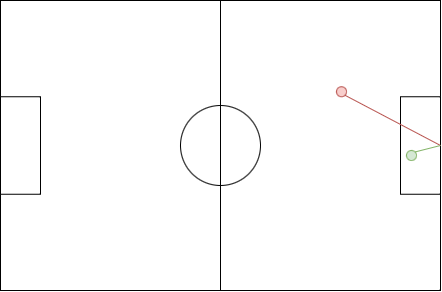
\includegraphics[width=7cm]{img/ExplicationXG.png}

    \caption{Emplacement de deux tirs sur un terrain de foot}
    \label{fig:expected_goal_example}
\end{figure}
\subsection{Intérêt de la problématique}
\noindent Cette problématique est très intéressante puisque c'est une donnée qui est dernièrement très populaire dans le monde du football. Elle donne plus d'informations sur le match que les autres statistiques d'un matchs (possession, nombre de passes, nombre de tirs cadrés, nombre de buts, etc.). Par exemple en ce qui concerne la possession, une équipe peut avoir la possession du ballon pendant 70\% du match mais ne pas marquer de buts, ni même être dangereuse avec le ballon. Le nombre de tirs cadrés, s'ils sont effectuées tous à l'extérieur de la surface de réparation, ne sont pas forcément dangereux. L'expected goal permet de donner une valeur à chaque tir et de déterminer si un tir a une chance d'être transformé en but.
\newline \newline
Certaines personnes utilisent cette métrique pour leurs paris sportifs. Ils observent la métrique lors des derniers matchs et la compare avec le score réel du match. Si la différence est grande, cela peut permettre de constater un manque de réalisme ou un sur-régime d'une des deux équipes. \cite{tennerelBienUtiliserExpected2022a}
\newline \newline
Les analystes de données des équipes utilisent cette donnée pour analyser les performances de leurs joueurs et de leurs équipes. Par exemple, la comparaison des xG et du nombre de buts marqués d'un joueur sur une période donnée peut permettre de déterminer la dangerosité et la capacité d'un buteur à terminer des actions. \cite{pettyWhatExpectedGoals2018a}
Les xG peuvent aussi être utilisés pour analyser les performances d'une équipe dans des situations bien précises. Une équipe qui possède un haut xG sur des contre-attaques montre qu'elle est très dangereuse sur ce type de situation. \cite{XGExplainedFBrefa}
L'une des choses les plus intéressante de cette métrique est qu'elle peut être utilisée pour analyser les forces et faiblesses des équipes. Par exemple, une équipe peut observer que ses xG sont très faibles lorsqu'elle tente des centres. Cela peut lui permettre de trouver son identité de jeu et de décider d'abandonner cette stratégie. Cette métrique est tout autant valable pour analyser les forces et faiblesses d'une équipe adverse. Dans la même situation, si une équipe vient à affronter l'équipe qui a dû mal à produire des xG sur des centres, elle peut décider de la forcer à jouer sur des centres en libérant de l'espace sur les côtés par exemple.
\newline \newline
Cette métrique est également utilisée pour aider les recruteurs à juger les performances de finition d'un joueur \cite{garratt-stanleyWhatExpectedGoals2022}. Nous avons vu précédemment qu'il existait des dérivées des xG comme les xA\footnote{Passes décisives attendues}. Les différentes dérivées peuvent permettre de juger les performances et qualités d'un joueur qui se trouve dans un poste bien précis. Par exemple, un milieu de terrain ou un défenseur peut être jugé sur ses xA et un attaquant sur ses xG.


\subsection{Questions que l'on souhaite répondre dans ce travail}
\noindent Il y a deux grandes questions à répondre dans ce travail.
\begin{itemize}
    \item Quels sont les paramètres qui influencent le plus l'expected goal ?
    \item Quel est le meilleur modèle pour prédire l'expected goal ?
\end{itemize}

\noindent Le but de ce travail est de comprendre quelles sont les variables qui influences le plus les xG.
Cela permettra de comprendre quelles sont les variables les plus importantes pour prédire les xG.
Grâce à cela, il est possible pour un analyste de données d'une équipe de football de savoir quelles sont les facteurs qui influencent le plus la qualité d'un tir.
Cela peut permettre de déterminer les forces et faiblesses d'une équipe et de savoir sur quels aspects travailler pour améliorer les performances de l'équipe.
\newline \newline
\noindent Le deuxième objectif de ce travail est de trouver le meilleur modèle pour prédire les xG.
En effet, le but sera d'avoir le modèle le plus performant et de comparer les différents modèles qui peuvent être utilisée pour établir cette métrique.
Il faut également veiller à ce que le modèle ne fasse pas de sur-apprentissage. Il est donc important de faire attention à la complexité du modèle et de trouver le meilleur compromis entre la complexité et la performance du modèle.

\section{Plan du document}
\noindent Concernant le déroulement de ce travail, il y a plusieurs étapes.
Tout d'abord, il y a la recherche des travaux existants sur le sujet.
Parmi les travaux existants, je vais chercher à savoir quels datasets ont été utilisées ainsi que les résultats obtenus.
Cela me permettra de comparer mes résultats avec les résultats obtenus dans les autres travaux.
\newline \newline
La suite sera de trouver un dataset avec les informations nécessaires pour implémenter le modèle.
Une fois ce dataset trouvé, il va falloir le documenter. En effet, il est important de comprendre ce que chaque attribut représente.
L'étape suivante est également importante puisque le but sera de visualiser les données.
Cela permettra de voir si les données sont exploitables et si elles sont cohérentes.
Cela pourra également nous indiquer si des biais seront présents dans le modèle.
\newline \newline
Une fois que les données sont documentées et visualisées, il va falloir les préparer.
En effet, il pourrait y avoir des données manquantes mais qui sont disponibles après un traitement.
Il pourrait également y avoir des données qui ne sont pas exploitables et qui doivent être supprimées.
Par exemple, l'ID de la base de données d'un tir pourrait être supprimée car il n'appporte rien pour la prédiction de l'expected goal.
\newline \newline
Ensuite, on pourra commencer à implémenter le modèle et observer les facteurs qui influencent le plus sa prédiction du xG.
C'est également à ce moment-là qu'il faudra comparer les différents modèles pour voir lequel est le plus performant pour prédire les xG.
Il sera également intéressant de voir quelles variables peuvent être ajoutées au modèle pour améliorer sa précision.


\section{Synthèse des travaux existants}
\label{sec:synthese}
\noindent Le premier travail repertorié sur les xG et la qualité d'un tir est celui de Richard Pollard, Jake Ensum et Samuel Taylor \cite{pollardEstimatingProbabilityShot2004}.
Dans ce travail datant de 2004, la seule information indiquée concernant le dataset est que les données proviennent de la Coupe du monde 1986 et de celle de 2002.
Le modèle a été implémenté en utilisant une régression logistique.
Le nombre de tirs répertoriées dans ce travail est de 1096.
La conclusion de ce travail est que les 3 facteurs les plus influents pour la prédiction des xG sont :
\begin{itemize}
    \item La distance entre le tireur et le but
    \item L'angle du but en fonction de la position du tir
    \item L'espace entre le tireur et le défenseur le plus proche
\end{itemize}
Le résultat final de l'analyse de la régression logistique de ce travail ressemble à cela.
\begin{table}[htp]
    \centering
    \begin{tabular}{|l|l|l|l|l|l|l|}
        \hline
        \textbf{Predictor} & \textbf{Coefficient} & \textbf{z} & \textbf{p} & \textbf{ratio} & \textbf{Lower} & \textbf{Upper} \\ \hline
        Constant           & 0.3771               & 1.20       & 0.229      &                &                &                \\ \hline
        Distance           & -0.1586              & -9.51      & 0.000      & 0.85           & 0.83           & 0.88           \\ \hline
        Angle              & -0.0222              & -3.81      & 0.000      & 0.98           & 0.97           & 0.99           \\ \hline
        Space              & 0.7991               & 3.22       & 0.001      & 2.22           & 1.37           & 3.62           \\ \hline
    \end{tabular}
    \caption{Résultat de la régression logistique du travail de Pollard, Ensum et Taylor}
\end{table}

\noindent Le deuxième travail est celui de Izzatul Umami, Deden Hardan Gutama et Heliza Rahmania Hatta \cite{umamiImplementingExpectedGoal2021}. 
Ce travail utilise les données de Wyscout des 5 championnats majeurs en Europe de la saison 2019-20. Ces derniers ont décidés de prendre comme données :
\begin{itemize}
    \item La distance
    \item L'angle
    \item Si le tir est un tir de la tête ou pas
\end{itemize}
Dans le dataset, 32000 tirs ont été utilisées pour la création du modèle.
Comme pour le travail précédent, la régression logistique a été utilisée.
Il est également indiqué qu'une séparation du dataset a été faite pour avoir des données d'entraînement et de tests.
Dans leurs tests du modèle, il est indiqué que le but est de faire de la classification pour de futures instances, il faut donc utiliser un seuil.
Suite à l'utilisation d'un seuil pour la classification, une matrice de confusion a été faite pour ensuite calculer la spécificité et la sensibilité du modèle.
Ce principe de sensibilité et spécificité permet de choisir la meilleure performance selon le contexte d'utilisation du modèle.
\begin{equation}
    Sensitivity = \frac{True Positive}{True Positive + False Negative}
\end{equation}
\begin{equation}
    Specificity = \frac{True Negative}{True Negative + False Positive}
\end{equation}
La sensibilité permet de voir la capacité du modèle à prédire correctement les tirs qui sont des buts.
De l'autre côté, la spécificité permet de voir la capacité du modèle à prédire correctement les tirs qui ne sont pas des buts.
Comme indiqué dans le travail de Umami, Gutama et Hatta, la spécificité est plus importante que la sensibilité selon le contexte.
Dans le cas où le modèle est utilisé pour prédire un cancer, nous allons chercher à avoir une meilleur sensibilité pour éviter de passer à côté d'un cancer. \cite{umamiImplementingExpectedGoal2021}
Cela leur permet de savoir comment choisir le seuil pour la classification.
En conclusion de leur travail, ils ont obtenu une sensibilité de 0.9671945701357466 et une spécificité de 0.19034406215316316 pour un seuil 0.02.
Ils indiquent finalement que le modèle de xG est plus performant si l'on prend la distance et l'angle en compte plutôt que de prendre uniquement la distance.
Un graphique ROC \footnote{Receiver Operating Characteristic} a été fait pour montrer la performance du modèle. Cela permet de comparer la sensibilité et la spécificité pour chaque seuil.
\newline\newline
Un autre travail qui fournit également du code est celui de David Sumpter \cite{sumpterFittingXGModel}. 
Le travail de ce dernier est de créer un modèle de xG en utilisant une régression logistique. 
Il utilise les données de Wyscout du championnat anglais de la saison 2017-18. 
Ce dernier explique étape par étape ce qui est effectué pour créer et améliorer son modèle.
Il y a également des pistes pour convertir les positions X et Y en distance et en angle.
Il commence par créer un modèle de xG en utilisant uniquement la distance. 
Par la suite, il le fait uniquement avec l'angle.
Ensuite, il utilise de multiples facteurs, comme la distance au carré ou encore l'angle multiplié par la position X du tir, pour créer son modèle et il produit un résumé de la régression logistique.

\begin{table}[htp]
    \centering
    \begin{tabular}{|l|l|l|l|l|l|l|}
    \hline
    \textbf{Predictor} & \textbf{coef} & \textbf{std err} & \textbf{z} & \textbf{P\textgreater{}|z|} & \textbf{{[}0.025} & \textbf{0.975{]}} \\ \hline
    Intercept          & -0.5103       & 0.887            & -0.576     & 0.565                       & -2.248            & 1.228             \\ \hline
    Angle              & -0.6338       & 0.319            & -1.989     & 0.047                       & -1.258            & -0.009            \\ \hline
    Distance           & 0.2798        & 0.118            & 2.381      & 0.017                       & 0.049             & 0.510             \\ \hline
    X                  & -0.1243       & 0.124            & -1.001     & 0.317                       & -0.368            & 0.119             \\ \hline
    C                  & 0.0300        & 0.040            & 0.750      & 0.454                       & -0.048            & 0.109             \\ \hline
    X2                 & -0.0014       & 0.001            & -1.422     & 0.155                       & -0.003            & 0.001             \\ \hline
    C2                 & -0.0041       & 0.003            & -1.398     & 0.162                       & -0.010            & 0.002             \\ \hline
    AX                 & 0.1251        & 0.118            & 1.063      & 0.288                       & -0.105            & 0.356             \\ \hline
    \end{tabular}
    \caption{Résumé de la régression logistique du modèle de xG de David Sumpter}
\end{table}
\noindent Il n'y a pas moyen de connaître les coefficients uniquement pour la distance et l'angle car aucun résumé n'est fait pour ces deux facteurs uniquement.
\newline\newline
Le dernier travail est fait par H.P.H Eggels. 
Le but est d'expliquer le résultat d'un match en utilisant les xG. 
Dans ce travail, il utilise un modèle de xG pour prédire le résultat d'un match.
Les données du travail proviennent de ORTEC, de Immotio et FIFA. En effet, son travail utilise trois datasets pour créer son modèle de xG. \cite{eggelsExpectedGoalsSoccer2016}.
Il y a eu un travail de "merging" des données pour avoir un dataset qui contient toutes les informations nécessaires pour créer le modèle. 
Cependant, les datasets peuvent avoir des problèmes entre eux lors du "merging". 
Par exemple, les noms des joueurs qui sont différents (majuscule, accent, encodage, surnom, etc.) a été un problème mais une solution a été trouvée.
\newline
Le dataset utilisé contient donc trois sources de données différentes.
\begin{table}[htp]
    \centering
    \begin{tabular}{lll}
    \hline
    \textbf{ORTEC}  & \textbf{FIFA}       & \textbf{Immotio}                  \\ \hline
    Context         & Player quality      & Number of attackers in line       \\
    Part of body    & Goal keeper quality & Number of defenders in line       \\
    Dist to goal    &                     & Distance nearest defender in line \\
    Angle to goal   &                     & Distance goal keeper              \\
    Originates from &                     &                                   \\
    Current score   &                     &                                   \\
    High            &                     &                                   \\ \hline
    \end{tabular}
    \caption{Sources de données utilisées par H.P.H Eggels}
\end{table}
\newpage
Parmi les modèles testés, ce travail utilise :
\begin{itemize}
    \item Un modèle de régression logistique
    \item Random Forest
    \item Un arbre de décision
    \item Ada-boost
\end{itemize}
Pour chacun de ces modèles, il y a une liste des différents paramètres qui vont être utilisés pour trouver le meilleur modèle.
Chacun des modèles a suivi une procédure avec un set d'entraînement, un set de validation et un set de test.
Le set de validation permet de trouver les meilleurs paramètres pour le modèle.
Le set de test permet de tester le modèle avec les paramètres trouvés et le comparer avec les autres modèles
Le modèle le plus performant parmi les quatres cités est le Random Forest avec une précision de 0.771.
Cependant, il n'est pas possible de connaître les meilleurs hyper paramètres pour chacun des modèles.
Ce travail donne tout de même de bonnes pistes pour l'ajout de nouvelle données pour améliorer le modèle de xG.


\subsection{Récapitulatif des travaux existants}
% Please add the following required packages to your document preamble:
% \usepackage[normalem]{ulem}
% \useunder{\uline}{\ul}{}
\begin{table}[htp]
    \centering
    \begin{tabular}{lll}
    \hline
    \textbf{Auteur(s)}                                                                                   & \textbf{Source de données}                                                                               & \textbf{Conclusion}                                                                                                                                          \\ \hline
    \begin{tabular}[c]{@{}l@{}}Richard Pollard\\ Jake Ensum\\ Samuel Taylor\end{tabular}                 & \begin{tabular}[c]{@{}l@{}}Coupe du monde \\ 1986 et 2002\end{tabular}                                   & \begin{tabular}[c]{@{}l@{}}La distance, l'angle \\ et l'espace avec le \\ joueur le plus proche\end{tabular}                                                 \\ \hline
    \begin{tabular}[c]{@{}l@{}}Izzatul Umami\\ Deden Hardan Gautama\\ Heliza Rahmania Hatta\end{tabular} & \begin{tabular}[c]{@{}l@{}}Wyscout, \\ 5 championnats \\ majeuren Europe. \\ Saison 2019-20\end{tabular} & \begin{tabular}[c]{@{}l@{}}La distance et l'angle\\ apporte plus \\ d'informations \\ qu'uniquement\\  la distance\end{tabular}                              \\ \hline
    David Sumpter                                                                                        & \begin{tabular}[c]{@{}l@{}}Wyscout, \\ Premier League.\\ Saison 2017-18\end{tabular}                     & \begin{tabular}[c]{@{}l@{}}La distance et l'angle \\ sont les facteurs avec\\  le plus d'influence\end{tabular}                                              \\ \hline
    H. P. H Eggels                                                                                       & \begin{tabular}[c]{@{}l@{}}ORTEC, \\ Immotio, \\ FIFA\end{tabular}                                       & \begin{tabular}[c]{@{}l@{}}Le but du travail \\ est de prédire les \\ résultats des matchs. \\ Rien n'indique les\\ facteurs les plus influents\end{tabular} \\ \hline
    \end{tabular}
    \caption{Récapitulatif des travaux existants}
\end{table}


\section{Dataset}

\subsection{Présentation du dataset}

\noindent Comme indiqué dans le section \ref{sec:synthese}, le travail de David Sumpter \cite{sumpterFittingXGModel} va être utilisé comme base pour implémenter le premier modèle. Il utilise un dataset qui contient les données de Wyscout. Wyscout est une entreprise qui fournit des données sur le football. Elle fournit des données sur les matchs, les joueurs, les équipes, les compétitions, etc. Il n'a pas été possible pour moi d'accéder aux données de Wyscout. J'ai donc utilisé un dataset public qui est un sample du dataset de Wyscout. \cite{pappalardoPublicDataSet2019}
\newline
\noindent Cette source permet d'avoir l'information des événements lors d'un match de foot, comme par exemple les passes, les tirs, les fautes, etc. Cela permet d'avoir les informations nécessaires pour calculer l'expected goal. Un autre avantage de ce dataset est qu'il est déjà nettoyé et qu'il est facilement utilisable. Il est aussi très complet puisqu'il contient des données sur les matchs de 5 championnats européens (Angleterre, Espagne, Italie, Allemagne et France) de la saison 2017-2018. Il contient aussi des données sur les matchs de la coupe du monde 2018 et de l'Euro 2016.

% Description de chaque attribut dans le dataset event
\subsection{Events}

% Description de chaque attribut dans le dataset players
\subsection{Players}

% Bibliography
\bibliographystyle{plain}
\bibliography{bibliography}

\end{document}